\section{Computation, certification, and reproducibility}
\label{sec:verification}

The proofs establish convergence and branch validity.  Computation has
a separate role: detecting arithmetic, phase, and branch mistakes in
the displayed examples.  The archive contains exact rational
coefficient generators and high precision checks; their numerical
outputs are not used as substitutes for the analytic arguments.

\subsection{A terminating coefficient calculation}

For a prescribed degree \(N\), the coefficient of \(Q^n\) in
a finite phase Euler product is computed by
\cref{eq:lambda-arithmetic,eq:euler-recurrence}.
For unphased integer products it can also be computed independently
by multiplying the finitely many relevant factors
\((1-Q^{dj})^{r_d}\), since factors with \(dj>N\) do not affect
that truncation.  Negative powers use the ordinary generalized
binomial coefficients.

Once the first surviving order \(\nu\) is known, form
\[
 H(Q)=\frac{R(Q)-1}{c_\nu Q^\nu}.
\]
Computing \(\Psi\) through degree \(N\) requires \(H\) only
through degree \(N-1\).  Computing \(\ell\) through degree \(N\)
requires \(H\) through degree \(N\).
Each rational-power coefficient is obtained from
\[
 (1+Z)^\alpha
 =\sum_{j=0}^N\binom{\alpha}{j}Z^j
 \pmod{Q^{N+1}},
\]
with a finite sum.
Exact composition then verifies
\(R(\Psi(u))=1+c_\nu u^\nu\) through the available order.

In the supplied program, both Euler-product methods agree,
the inverse compositions agree exactly, and the arbitrary-order
four-factor balances and primitive vectors are checked for
\(m=1,\ldots,7\).
These checks target independent representations of the formulas.

\subsection{A concrete certified disk for the eta example}

The hypotheses of \cref{thm:flat-tail} can be verified with
rational inequalities, not merely numerical sampling.
For \cref{eq:R2}, put
\(H(Q)=(1-R_2(Q))/(3Q^2)\), and choose \(r=1/20\).
On \(|Q|=r\), let
\begin{align*}
 E_r&=
 3\,\frac{r^4(2-r^2)}{(1-r^2)^2}
 +4\,\frac{r^3}{(1-r^3)^2}
 +\frac{r^6}{(1-r^6)^2},\\
 T_r&=3r^2+E_r .
\end{align*}
The first quantity bounds
\(|\log R_2(Q)+3Q^2|\): in the \(P(Q^2)^3\)
term use \(\sigma_{-1}(n)\le n\) after removing degree two.
The other two factors use \cref{eq:log-product-bound}.
Consequently \(|\log R_2|\le T_r<1\), and
\[
 |R_2-1-\log R_2|
 \le \tfrac12 T_r^2\ee^{T_r}
 \le \frac{T_r^2}{2(1-T_r)}.
\]
The maximum-modulus principle applied to the removable analytic
function \(H-1\) gives
\begin{equation}\label{eq:explicit-H-bound}
 \sup_{|Q|\le r}|H(Q)-1|
 \le \frac{E_r}{3r^2}
      +\frac{T_r^2}{6r^2(1-T_r)}
 <\frac12.
\end{equation}
The final comparison is an exact rational inequality; its
left side bound is approximately \(0.0760461945891084\), and the
supplied rational-arithmetic calculation proves that it is less than
\(760463/10^7<1/2\).
Thus \(R_0=1/(20\sqrt2)\) and \(M=(\log2)/2\)
are explicit valid constants in \cref{thm:flat-tail}.
The numerical cutoff is conservative, but it is completely
reviewable.

For numerical evaluation of a dual factor, truncating
\(P(z)\) after \(J\) factors has logarithmic tail bounded by
\begin{equation}\label{eq:product-tail}
 \left|\sum_{n>J}\log(1-z^n)\right|
 \le
 \frac{|z|^{J+1}}
 {(1-|z|)(1-|z|^{J+1})}.
\end{equation}
Indeed expand each logarithm, sum the geometric tail in \(n\),
and bound \(1-|z|^\ell\) below by \(1-|z|\).
A sum of these bounds, weighted by the absolute factor exponents,
controls a quotient's logarithm.
To convert a logarithmic error \(\varepsilon\) to relative
multiplicative error, use
\(|\ee^\varepsilon-1|\le|\varepsilon|\ee^{|\varepsilon|}\).

\subsection{Numerical examples and logarithm winding}

The principal eta inverse \cref{eq:eta-example-Q}
was evaluated at 360 decimal digits.
The following table uses the polynomial for \(Q(s)\) through
degree \(10\), followed by the coherent logarithm
\(t=(2\pi^2/3)/(-\log Q)\).
It therefore reports a \(Q\)-polynomial truncation, rather than
the \(\ell\)-polynomial truncation in \cref{eq:flat-certified}.

\begin{center}
\begin{tabular}{@{}cc@{}}
\toprule
Original parameter \(t\) & Observed absolute inverse error\\
\midrule
\(0.8\) & \(3.33249\times10^{-35}\)\\
\(0.5\) & \(4.82563\times10^{-57}\)\\
\(0.3\) & \(1.37812\times10^{-95}\)\\
\(0.5+0.15\ii\) & \(2.75344\times10^{-52}\)\\
\bottomrule
\end{tabular}
\end{center}

The complex example requires logarithmic winding index \(-1\)
when its nome is first represented with the principal logarithm.
Resetting that logarithm would return a different inverse sheet.
At the same output as \(t=0.8\), the other small nome root
gives, on one logarithm lift,
\[
 t_-\approx
 0.6981170734058837+0.2666494981906634\,\ii .
\]
Direct evaluation of the original eta quotient agrees for these
two parameters to the working numerical precision.
The existence of both branches follows from
\cref{thm:flat-inverse}; the computation verifies the sheet
bookkeeping in a concrete case.

\begin{figure}[htbp]
 \centering
 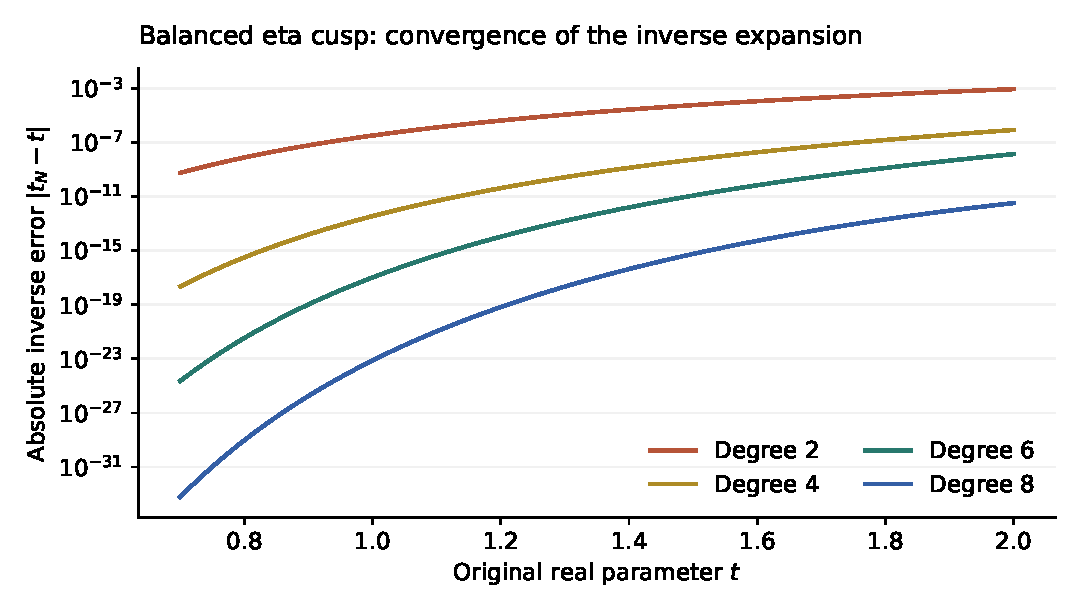
\includegraphics[width=.96\textwidth]{figures/eta_inverse_convergence.pdf}
 \caption{Observed error after truncating the nome inverse \(Q(s)\)
 at degrees \(2,4,6,8\), then taking a coherent logarithm.
 Each curve uses direct high precision evaluation of the eta example.
 Moving toward the cusp makes the exponential coordinate smaller.
 The curves are numerical illustrations; the analytic tail bounds
 are \cref{eq:flat-certified,eq:product-tail}.}
 \label{fig:convergence}
\end{figure}

The archive also records the rational \(q\)-gamma product
checks for \(k=2,3,4\), the four-factor family at real and
complex arguments, explicit rational-cusp phase checks, and
paired-term Stokes contour checks.
The latter compare the two directional integrals with their
residue sum; the counterexample itself is established by its
contour proof, independently of those calculations.

The supplementary phase program checks 24 one-factor and 24
general-product identities, with both real and complex parameters,
at 80 decimal digits.  The largest scaled residual is less than
\(1.3\times10^{-79}\).  It also checks Dedekind reciprocity with
exact rational arithmetic and records the rational certificate in
\cref{eq:explicit-H-bound}.
The Stokes program independently integrates four paired summands
along the two rays; each difference agrees with its residue sum to
absolute error less than \(4\times10^{-82}\).
These are reproducible checks at specified working precision;
the numerical residuals are not interval-arithmetic certificates.

\subsection{An implementation procedure}

A reliable implementation can follow this sequence.
\begin{enumerate}[leftmargin=*,itemsep=3pt]
\item Record the input function, variable being inverted, cusp,
      target normalization, sector, and logarithm lift.
\item For a finite eta or Euler quotient, compute
      \(g_d,\rho_d,A_{h,k},B,D\) exactly.
      Select the appropriate core regime.
\item Combine coincident action coefficients in a cyclotomic
      field before identifying the first surviving term.
\item Use the exact-core theorem, the finite-endpoint scale,
      or the flat-cusp inverse according to that regime.
      Near a zero of the core derivative, change the local chart.
\item Generate coefficients to the desired order, verify
      composition algebraically, and compute a disk or tail bound.
\item Evaluate products through the dual nome, preserving
      logarithm lifts.  If the target comes from a Borel sum,
      carry the contour's residue correction into the equation.
\end{enumerate}

This procedure makes two common failure modes explicit.
Deleting a flat modular factor may remove the entire inverse
problem after balancing.  Ignoring a Stokes correction may
invert a different sectorial function while preserving the same
formal power series.

\section{Further research questions and precise remaining boundaries}
\label{sec:future}

The article supplies exact results for substantial classes, but a
general complex transseries program has additional problems.
The following questions separate those problems by the missing
mathematical ingredient.

\begin{question}[Uniform parameter-dependent resurgent inversion]
Starting with \cref{eq:cb-borel}, prove the full family of
resurgent seminorm bounds needed for implicit inversion in
\(a\), uniformly on compact subsets of \(|a|<1\), with specified
contours and target jumps.  Identify a natural function space in
which both the contour correction and the inverse depend
holomorphically on the parameters.
\end{question}

The meromorphic Borel transform and the exact equation
\cref{eq:cb-inverse-exact} are available.
A pointwise nonzero derivative does not by itself supply uniform
inverse radii or all of the needed functional analytic estimates.
This is the part of the repository's implicit conjecture that
has not been replaced here by an unconditional general theorem.

\begin{question}[Coalescing fixed-argument and modular limits]
Obtain a uniform inverse theory when \(a=a(t)\) approaches the
unit circle, for example \(a(t)=\ee^{-\alpha t}\), while
\(q=\zeta\ee^{-t}\to\zeta\).
How do the Borel pole arrays reorganize into the modular
completions when \(\alpha\) is rational, and what replaces those
completions for general complex \(\alpha\)?
\end{question}

The fixed compact-\(a\) estimates deteriorate as \(|a|\to1\).
The exact eta and rational \(q\)-gamma identities avoid that
deterioration in special cases but do not prove a uniform
transition theorem for arbitrary \(\alpha\).
A useful first goal is a two-parameter sector with an explicit
matching estimate on an overlap.

\begin{question}[Moving cusps with growing denominator]
For fixed dilations and rational cusps \(h/k\) depending on \(t\),
determine uniform reversion and error bounds across the
transition \(k^2t\asymp1\), including the phase arithmetic.
\end{question}

The exact normal form remains valid.
What fails is the conclusion \(Q\to0\).
A transition approximation must retain a non-small dual product,
and cannot follow from a finite number of its coefficients.
Uniform control in \(h\) and \(k\) is a separate issue from
the fixed-cusp formula.

\begin{question}[Effective cancellation certificates]
Given a finite phase Euler product, find practical bounds on
the first nonzero coefficient of its logarithm, or prove that
it is identically zero.
Can modular-form bounds and arithmetic coefficient recurrences
be combined to outperform direct expansion, including products
with nontrivial eta multipliers?
\end{question}

The constructions here have visible first coefficients.
For arbitrary phase products, cancellation can be extensive or
complete.  An effective certificate should also identify the
primitive action lattice, so that a reported ramification
order is intrinsic to the chosen minimal nome.

\begin{question}[Optimal level and height for a prescribed ramification]
Among all balanced products realizing order \(m\), minimize
the common level, the largest original dilation, or the sum of
the absolute exponents.  Determine the tradeoff between those
quantities under two versus three balance constraints.
\end{question}

The factor counts three and four are sharp.
They do not optimize the level of the four-factor construction,
which uses an lcm of four consecutive integers.
The one-dimensional classification
\cref{eq:four-support-classification} supplies an exact starting
point for the optimization.

\begin{question}[Global continuation and coefficient asymptotics]
For a specific balanced quotient, locate the first singularities
of \(\Psi(u)\), including critical values of the dual product
and images of other cusps.  Determine the exact convergence
radius and the large-order asymptotics of its inverse coefficients.
\end{question}

The local inverse theorem gives a positive radius, not its
optimal value.  Modular coordinates may permit a global analysis
in low-level examples.  Such an analysis requires a verified
description of the relevant modular curve or covering and should
not be inferred from a few inverse coefficients.

\begin{question}[Unfolding a flat critical point]
Let a parameter break one or more balance equations, so that
\[
 F_\varepsilon(t)=
 C\,t^{-b(\varepsilon)}
 \ee^{-a(\varepsilon)/t+c(\varepsilon)t}
 R_\varepsilon(\ee^{-S/t}).
\]
Construct uniform inverse charts as the algebraic core and the
flat defect become comparable.
\end{question}

Theorems for each separate regime do not automatically remain
uniform when \(a,b,c\to0\).
Natural transition variables compare
\(a/t\), \(b\log t\), and \(ct\) with
the first surviving \(Q\)-action.
This is a singular perturbation problem rather than an ordinary
fixed-parameter application of the inverse-function theorem.

\begin{question}[Finite moving critical points and higher multiplicity]
Extend the present exact examples to a parameter-dependent
critical point of multiplicity \(m\), with explicit moving
discriminants, sheet radii, and crossover bounds.
\end{question}

The generic local Puiseux theorem is already available in the
repository.  A perturbed critical point may split.
For instance \(u^2+\varepsilon u=y\) has its critical value at
\(-\varepsilon^2/4\), so an expansion about the undeformed
critical value is not uniform.
The arbitrary-\(m\) cusp constructions do not solve that
full moving-discriminant problem.

\begin{question}[Infinite and accumulating complex actions]
Replace the finite analytic action set by a countable one,
possibly with accumulation in exponential height.
Find conditions under which coefficient grouping, analytic
substitution, and inverse summation remain compatible.
\end{question}

The finite decay-cone argument bounds the number of indices at
each height.  It does not extend merely by writing an infinite
list of actions.  A viable theorem needs quantitative summability
of grouped coefficients and control of the inverse iteration.

\begin{question}[More \(q\)-special functions and joint criticality]
Determine which rational combinations of \(q\)-beta,
\(q\)-gamma, \(q\)-Barnes functions, and Gaussian coefficients
admit exact modular completions with enough balance to create
flat critical values.  Study joint argument/base critical limits.
\end{question}

The product identities in \cref{sec:qgamma} provide a
testable model: first isolate an exact analytic background, then
identify the surviving modular coordinate and apply the
appropriate inverse theorem.
Existing questions on optimal \(q\)-multinomial truncation,
pole pinching, and the motion of the \(q\)-gamma minimum remain
distinct \cite{repo-qsharp,repo-qmono}.

\begin{question}[Formal verification of the analytic boundary]
Formalize the finite arithmetic recurrences and balance
constructions, then connect them to a verified analytic
inverse theorem and explicit complex product bounds.
\end{question}

The rational coefficient generator is a suitable first target.
A full proof also needs complex branch data, normal convergence,
Rouch\'e or contraction certificates, and the modular identity.
No theorem in this article is claimed to have been checked by
a proof-assistant kernel.  The included programs check exact
finite algebra and numerical examples.

\subsection{What is settled here}

The directional-equality assertion in the named repository
conjecture has an explicit counterexample, while its
fixed-argument Gevrey and Borel-continuation content has a
direct, literature-consistent proof.
The complete-cancellation question has explicit arbitrary-order
examples with sharp factor counts.
The inverse charts have all coefficients, all small-nome
logarithmic sheets, and quantitative tails.
The rational \(q\)-gamma applications distinguish the flat
normalized inverse from the regular-core inverse of the original
observable.

These conclusions are compatible with the limits stated
throughout: fixed sectors and branches are part of the data;
a fixed-cusp formula is not a growing-denominator theorem;
local convergence is not global continuation; and a finite
analytic action model is not the entire field of complex
transseries.
